%-------------------------------------------------------------------------------------------------------
%-------------------------------------------------------------------------------------------------------
% Sec & Label

\section{Theoretical Analysis}
\label{sec:analysis}


%-------------------------------------------------------------------------------------------------------
%-------------------------------------------------------------------------------------------------------
% Intro

In this section we will explain the inner workings of the band-pass filter created and perform a theoretical analysis of each component. 
The voltage divider law was used in cunjunction to the OP-Amp non-inverting amplifier configuration. 

%-----------------------------------------------------------------------
%-----------------------------------------------------------------------
% 		     	    Transf - subsec
% ----------------------------------------------------------------------
% ----------------------------------------------------------------------

\subsection{High-Pass Filter}
\label{subsec:transf}

The first stage of the of the band-pass filter is comprised of a High-Pass filter. It is in this stage that the low cut-off frequency is set.

In this stage a combination of a resistor and a capacitor with specific values is set in a way as to have a gain of almost unity for frequencies above a certain threshold (100Hz in our circuit).

Gain of High-Pass filter:

\[
\frac{V_o}{V_{in}} = \frac{R_3}{\sqrt[2]{R_3+\frac{1}{\omega C}}}
\]

with \(R\) being the resistor value, and \(\frac{1}{wC}\) the absolute value of the impeadance of the capacitor (with \(\omega\) as angular frequency and \(C\) the capacitor capacitance).

The treshold frequency is set by the following equation:
\[
f = \frac{1}{2\pi f}
\]

\subsection{OPAMP: Non-inverting amplifier}
\label{subsec:envdet}

It is in this stage that the amplification of the signal takes place. At the same time this stage works as a low-pass filter.

The signal amplification is dependent on the ratio of the two resistances (\(R_1\) and \(R_2\) by the following expression:
\[
\frac{V_o}{V_{in}} = 1 + \frac{R_2}{R_1}
\]

Due to the internal composition of the OP-Amp it also works as the low-pass filter used in the circuit and it set the high cut-off frequency. Since the theoretical octave script assumes a perfect OP-Amp, the cut-off frequency won't exist.


\subsection {Circuit frequency response}
Due to the use of a capacitor in the circuit, the gain is dependent on the frenquecy of the imput. This response was achieved by calculating the equivelent impedance of the stage with a capacitor for a set of frequencies.

%\begin{figure}[ht]
%	\centering
%	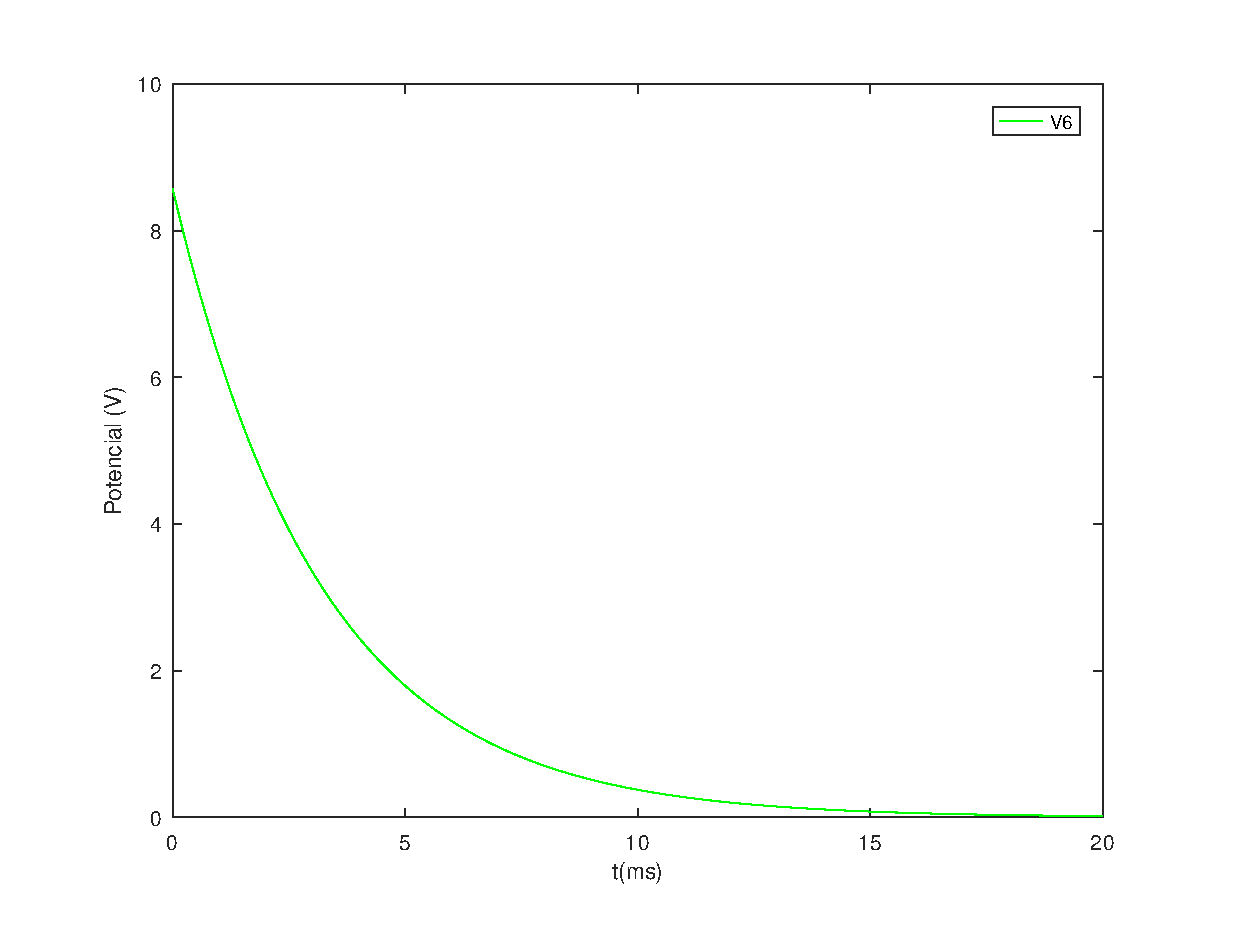
\includegraphics[width=0.7\linewidth]{plot1.eps}
%	\caption{Frequency Response Vo/Vi.}
%\label{fig:oct}
%\end{figure}

%-----------------------------------------------------------------------
%-----------------------------------------------------------------------
% 			     Results - subsec
% ----------------------------------------------------------------------
% ----------------------------------------------------------------------

\subsection{Theoretical Results}
\label{subsec:res_the}

The obtained results were as follows:
\begin{figure}[ht]
	\centering
	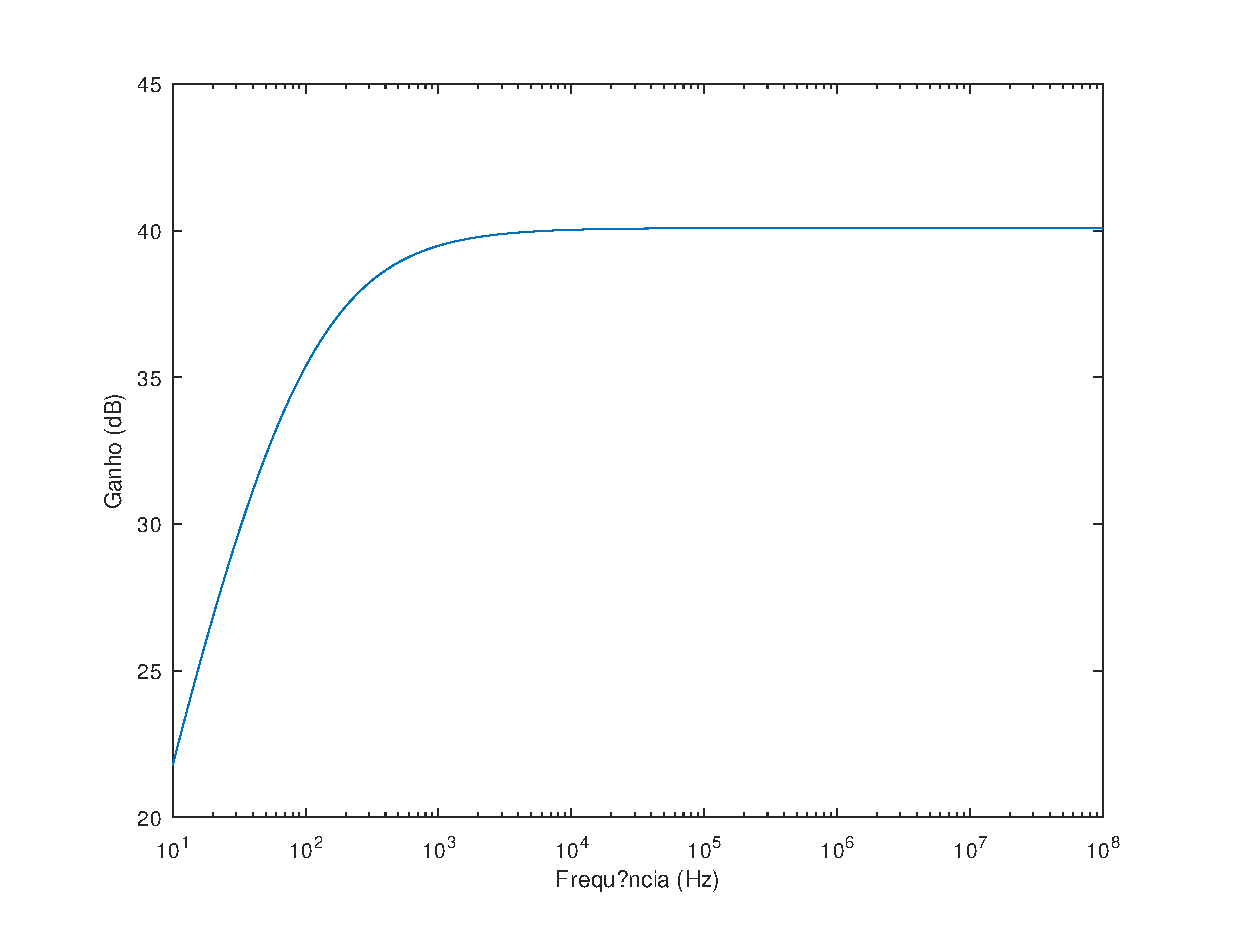
\includegraphics[width=0.7\linewidth]{band_pass.eps}
	\caption{Frequency Response Vo/Vi.}
\label{fig:oct}
\end{figure}

%\begin{table}[ht]
%	\centering
%	\begin{tabular}{|l|r|}
%		\hline    
%		{\bf Name} & {\bf Value} \\ \hline
%   		$Ve$ & 1.093271e+00 \\ \hline 
$Vc$ & 9.912854e+00 \\ \hline 
$Vce$ & 8.819583e+00 \\ \hline 
$Vec2$ & 1.061285e+01 \\ \hline 

%	\end{tabular}
%	
%	\caption{Values from Octave.}
%   
%\label{tab:op_teo}
%\end{table}

%\begin{table}[ht]
%	\centering
%	\begin{tabular}{|l|r|}
%		\hline    
%		{\bf Name} & {\bf Value[Ohm]} \\ \hline
%   		$Z1_{In}$ & 8.064050e+03 \\ \hline 
$Z1_{Out}$ & 9.951958e+02 \\ \hline 
$Z2_{In}$ & 8.598855e+03 \\ \hline 
$Z2_{Out}$ & 3.021730e-01 \\ \hline 
$Zt_{Out}$ & 4.411395e+00 \\ \hline 

%	\end{tabular}
%	
%	\caption{Values from Octave.}
%\label{tab:imp_teo}
%\end{table}


